\usetikzlibrary{arrows.meta}
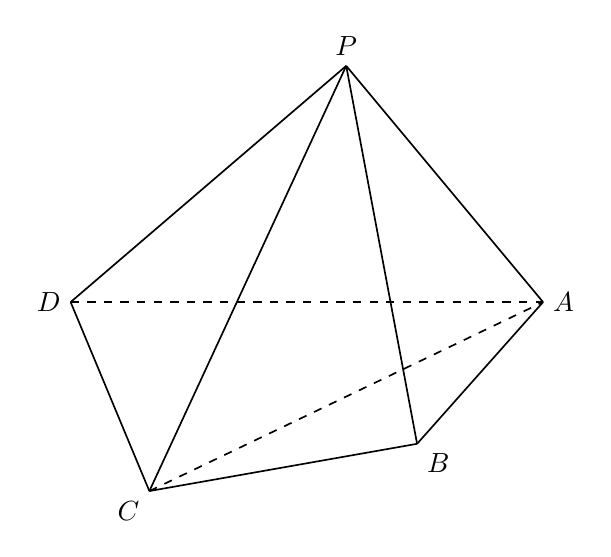
\begin{tikzpicture}[x=1cm,y=1cm,line width=.6pt,font=\normalsize,>=Stealth]
\coordinate (P) at (0.5,3.2);
\coordinate (D) at (-3,0.2);
\coordinate (A) at (3,0.2);
\coordinate (C) at (-2,-2.2);
\coordinate (B) at (1.4,-1.6);
% visible solid edges
\draw[solid] (P)--(D);
\draw[solid] (P)--(C);
\draw[solid] (P)--(A);
\draw[solid] (P)--(B);
\draw[solid] (D)--(C);
\draw[solid] (C)--(B);
\draw[solid] (A)--(B);
% hidden dashed edges
\draw[dashed] (D)--(A);
\draw[dashed] (C)--(A);
\node[above] at (P) {$P$};
\node[left] at (D) {$D$};
\node[right] at (A) {$A$};
\node[below left] at (C) {$C$};
\node[below right] at (B) {$B$};
\end{tikzpicture}
